\section{Langkah-Langkah Percobaan}
Bagian ini menjelaskan secara rinci tahapan atau prosedur yang dilakukan selama praktikum. Langkah-langkah ditulis secara urut dan sistematis, mulai dari persiapan alat hingga pelaksanaan percobaan. Penulisan harus jelas agar dapat dipahami oleh orang lain yang membaca laporan ini.

\section{Analisis Hasil Percobaan}
Berisi pembahasan terhadap hasil yang diperoleh selama praktikum. Analisis dilakukan dengan membandingkan hasil percobaan terhadap teori, serta mengidentifikasi faktor-faktor yang memengaruhi hasil, seperti kesalahan alat atau langkah percobaan. Tujuan bagian ini adalah untuk mengevaluasi keberhasilan percobaan dan memastikan pemahaman praktikan terkait praktikum yang telah dilaksanakan.

\section{Hasil Tugas Modul}
\begin{enumerate}
  \item Berdasarkan tugas pendahuluan pada laporan sementara, berikut ini merupakan simulasi di cisco packet tracer \\
  	\begin{figure}[H] 
    \centering
    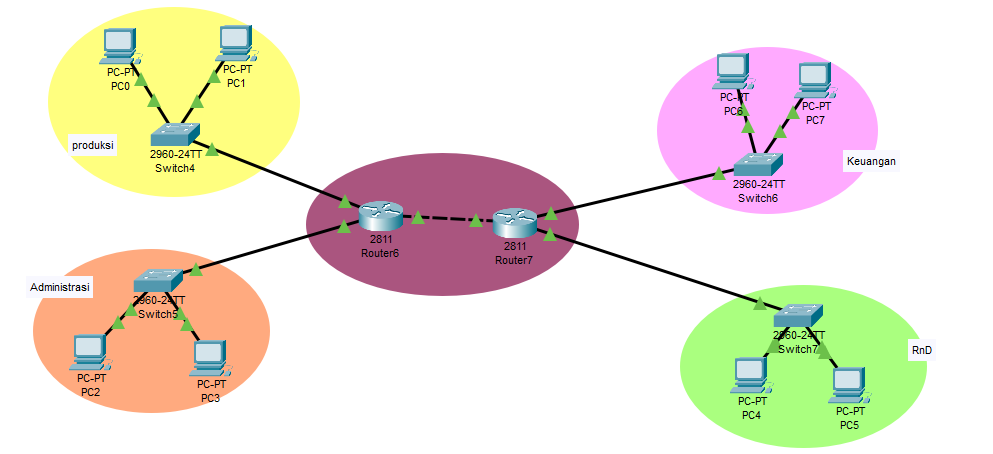
\includegraphics[width=0.5\textwidth]{P1/img/tupen3.png}
    \caption{Simulasi pada Cisco Packet Tracer}
    \label{fig: Simulasi pada Cisco Packet Tracer}
	\end{figure}
  Simulasi yang digunakan sebagaimana dapat dilihat di file \href{run:P1.pkt}{P1.pkt} [Lihat folder P1 > P1.pkt]
  \item 
  Selama praktikum, tantangan pertama  yang dihadapi adalah ketidakfamiliaran. Karena praktikan baru pertama kali melakukan crimping dan baru pertama kali juga melakukan konfigurasi untuk router mikrotik. Praktikan juga sempat bingung router mana dan interface mana yang harus memakai alamat.
\end{enumerate}

\section{Kesimpulan}
Kesimpulan berisi ringkasan dari hasil praktikum dan hal-hal penting yang didapatkan. Bagian ini menjawab tujuan praktikum, mencantumkan hasil yang sesuai atau tidak sesuai dengan teori, serta pembelajaran yang diperoleh oleh praktikan.

\section{Lampiran}
\subsection{Dokumentasi saat praktikum}
Menampilkan foto selama pelaksanaan praktikum. Dokumentasi meliputi foto alat yng digunakan dan foto praktikan saat praktikum. Tujuannya sebagai bukti telah dilakukan kegiatan praktikum.

\subsection{Hasil Challenge Modul}
Challenge pada praktikum ini adalah membuat mengembangkan konfigurasi dari praktikum dengan tambahan 2 switch (router yang dibuat menjadi switch) dan perubahan ukuran subnet menjadi untuk 100 perangkat dan 200 perangkat. 
